\begin{block}{Problem Statement}
  Alex holds two credit cards:
  \begin{itemize}
    \item \textbf{Card A}: Balance = \$1,800, Limit = \$4,000
    \item \textbf{Card B}: Balance = \$600, Limit = \$6,000
  \end{itemize}
  Calculate Alex's \textbf{overall credit utilization ratio} across both accounts.
\end{block}

\vspace{0.5em}
\centering
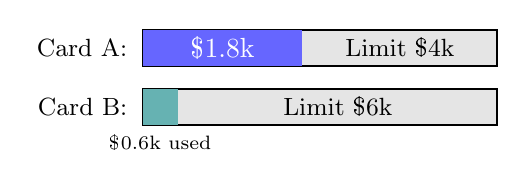
\begin{tikzpicture}[scale=0.75]
  % Card A
  \draw[thick, fill=gray!20] (0,1) rectangle (6,1.6);
  \fill[blue!60] (0,1) rectangle (2.7,1.6);
  \node[left] at (-0.1,1.3) {\small Card A:};
  \node at (1.35,1.3) {\color{white}\$1.8k};
  \node at (4.35,1.3) {\small Limit \$4k};

  % Card B
  \draw[thick, fill=gray!20] (0,0) rectangle (6,0.6);
  \fill[teal!60] (0,0) rectangle (0.6,0.6);
  \node[left] at (-0.1,0.3) {\small Card B:};
  \node[below] at (0.3,0) {\scriptsize \$0.6k used};
  \node at (3.3,0.3) {\small Limit \$6k};
\end{tikzpicture}
